\section{Synopsis}

Code coverage is a common technology for safety critical application which
permits to analyze how well an application is tested.
The technique used consists of inserting during the compilation
measurement points which permit tracking the execution of the source code. 

Several levels of instrumentation are available, the most common being:
\begin{description}
  \item[Line coverage]      instrumenting the execution per source code line. 
  \item[Branch coverage]    instrumenting the execution of each branching block. 
  \item[Decision coverage]  instrumenting each boolean decision of loop
    and selection statements.
  \item[Condition coverage] instrumenting of each sub-expression of boolean
    expressions.
\end{description}

\section{{\TestCocoon} and it's usage}

{\TestCocoon} is an open source code coverage tool for C++ code like GNU gcov,
but different in many ways. For example, \TestCocoon:
\begin{itemize}
  \item  works on release and debug build mode.
  \item  uses generic code, and is independent of compiler.
  \item  instrumentation is on the branch, decision and condition
    level, whereas gcov is limited to line coverage.
  \item  provides a graphical code browser.
  \item  records an instrumentation report for each test run. This
    permits you to compare or merge them.
  \item allows adding code coverage reports from unit tests
   into the instrumentation of main application. 
  \item permits you to measure work on the modified code between two
   software releases. 
  \item  support black box testing.
  \item  provides an extension to instrument {\Qt} source code, but not
   the unnecessary Qt infrastructure.
\end{itemize}


{\TestCocoon} is composed of 2 main tools:
\begin{description}
  \item[{\CoverageScanner}] {\CoverageScanner} is a easy to use compiler wrapper which
    instruments the source code just before calling the native compiler. In
    other words, it's a compiler replacement which produces an instrumented
   code. Unlike other tools, it does not require path insertion techniques,
   rather, telling the make tool to use it as an alternative compiler.
  \item[{\CoverageBrowser}] Code coverage visualization and analysis tool.
\end{description}

During the compilation, an instrumentation database is generated for each
object, library and executable. This database contains  a copy of the source
code, the instrumentation points, once executed, all test reports.

\section{Getting started with {\Qt} {\TextEdit} sample}

We will take \Qt's \TextEdit\ sample and use it to illustrate how \TestCocoon\ can be
involved at different stages of the development process.
To cover the coding cycle, we will first generate the instrumented application,
then perform manual tests and analyse their results, and finally we will create an
instrumented unit test.
In the second step we will  cover parts which are more of interest to product
management: analysis of impact of code corrections, tracking their test
progress, externalising testing and collecting the code coverage analysis of a
complete testing team.

\NOTE{\sloppy The modified \TextEdit\ sample can be downloaded from \url{http://testcocoon.org/texteditsample.tgz}.
The \Qt\ framework can directly be downloaded from \url{http://qt.nokia.com}.}

\subsection{Installing {\TestCocoon}}

Installing {\TestCocoon} is straightforward: just download the binaries  from
\url{http://testcocoon.org/download.html} and execute the installer.

\subsection{Compiling {\TextEdit}}

For the instrumentation generation it is simply a case of adapting the
\qmake\ project in order to add a new build configuration. Compiling the
application will then consist of executing:

\begin{center}
\begin{tabular}{|p{7cm}|p{7cm}|} \hline
  On Linux & On Windows \\\hline
\begin{alltt}
qmake CONFIG+=TestCocoon
make
\end{alltt}
&
\begin{alltt}
qmake CONFIG+=TestCocoon
nmake
\end{alltt} \\ \hline
\end{tabular} 
\end{center} 

Before modifying the project file, we need to ensure that the precompiled
headers are disabled. This is already the case for the {\TextEdit} sample.

In the {\TestCocoon} configuration, we first need to modify the compiler and linker
used in order to have {\CoverageScanner} instead of the native compiler. {\CoverageScanner}'s
wrapper executable name is the compiler name with the prefix cs. So we simply
add the following lines to \texttt{textedit.pro} to add instrumentation:

\begin{figureenv}
\begin{verbatim}
TestCocoon {
 QMAKE_CC=cs$$QMAKE_CC
 QMAKE_LINK=cs$$QMAKE_LINK
 QMAKE_CXX=cs$$QMAKE_CXX
}
\end{verbatim}
\caption{Minimal {\qmake} configuration}
\label{lst:qmake1}
\end{figureenv}

This should be sufficient for most applications, but for {\Qt} applications we need to
specify some additional parameters in order to skip the instrumentation of the
source code generated by {\Qt} tools (\uic, \qrc\ and \moc\ compiler).

To exclude instrumenting \qrc\ resources files, we simply tell CoverageScanner to
exclude from the instrumentation
every source file starting with qrc\_.
The command line option \verb$--cs-exclude-file-regex=qrc_.*$ achieves this.
Also, files generated using \uic\ can be excluded using the same command line
option: \verb$--cs-exclude-file-regex=ui_.*$ .

{\TestCocoon} also provides a command line switch dedicated to Qt4 applications
(\verb$--cs-qt4$). This permits:
\begin{itemize}
  \item skipping the instrumentation of the \verb$Q_OBJECT$ and
    \verb$Q_DECLARE_PLUGIN$ macros.
  \item skipping the engine code from the \moc\ compiler.
    This achieves only instrumenting the emission of signals and the reception
    of slots. 
\end{itemize}

We can choose also to count the execution of code (\verb$--cs-count$ command line
option) and do a full instrumentation at decision/condition
level(\verb$--cs-full-instrumentation$ command line option). The command line
option \verb$--cs-output$ permits to set the output file of the execution
report generated upon the application exit.



So, the final {\TestCocoon} configuration looks as follows:
\begin{figureenv}
\begin{verbatim}
TestCocoon {
 TESTCOCOON_OPTIONS =  --cs-count --cs-full-instrumentation
 TESTCOCOON_OPTIONS += --cs-qt4
 TESTCOCOON_OPTIONS += --cs-output=textedit
 TESTCOCOON_OPTIONS += --cs-exclude-file-regex=qrc_.*

 QMAKE_CXXFLAGS += $$TESTCOCOON_OPTIONS
 QMAKE_CCFLAGS  += $$TESTCOCOON_OPTIONS
 QMAKE_LFLAGS   += $$TESTCOCOON_OPTIONS

 QMAKE_CC=cs$$QMAKE_CC
 QMAKE_LINK=cs$$QMAKE_LINK
 QMAKE_CXX=cs$$QMAKE_CXX
}
\end{verbatim}
\caption{Final {\qmake} configuration}
\label{lst:qmake2}
\end{figureenv}

Compiling {\TextEdit} produces of course the \texttt{textedit.exe} executable and an additional file
\texttt{textedit.exe.csmes}, this is the  instrumentation database.

\subsubsection{First code coverage result}

We will start our first exercise by executing {\TextEdit} and then quitting the application immediately. A file called
\texttt{textedit.csexe} is generated.  Do not try to read it, it contains a binary
snapshot of the last execution run.

\sloppy Next step is to  start {\CoverageBrowser} and load \texttt{textedit.exe.csmes} instrumentation database
(Menu: \GUIMenuTwo{File}{Open\ldots}).  At this state, no coverage information is available
because no execution reports have been  imported. The instrumented code lines are
grayed-out and coverage statistics have not been computed. \seefigref{fig:startup}

\begin{figure}[H]
  \begin{center}
    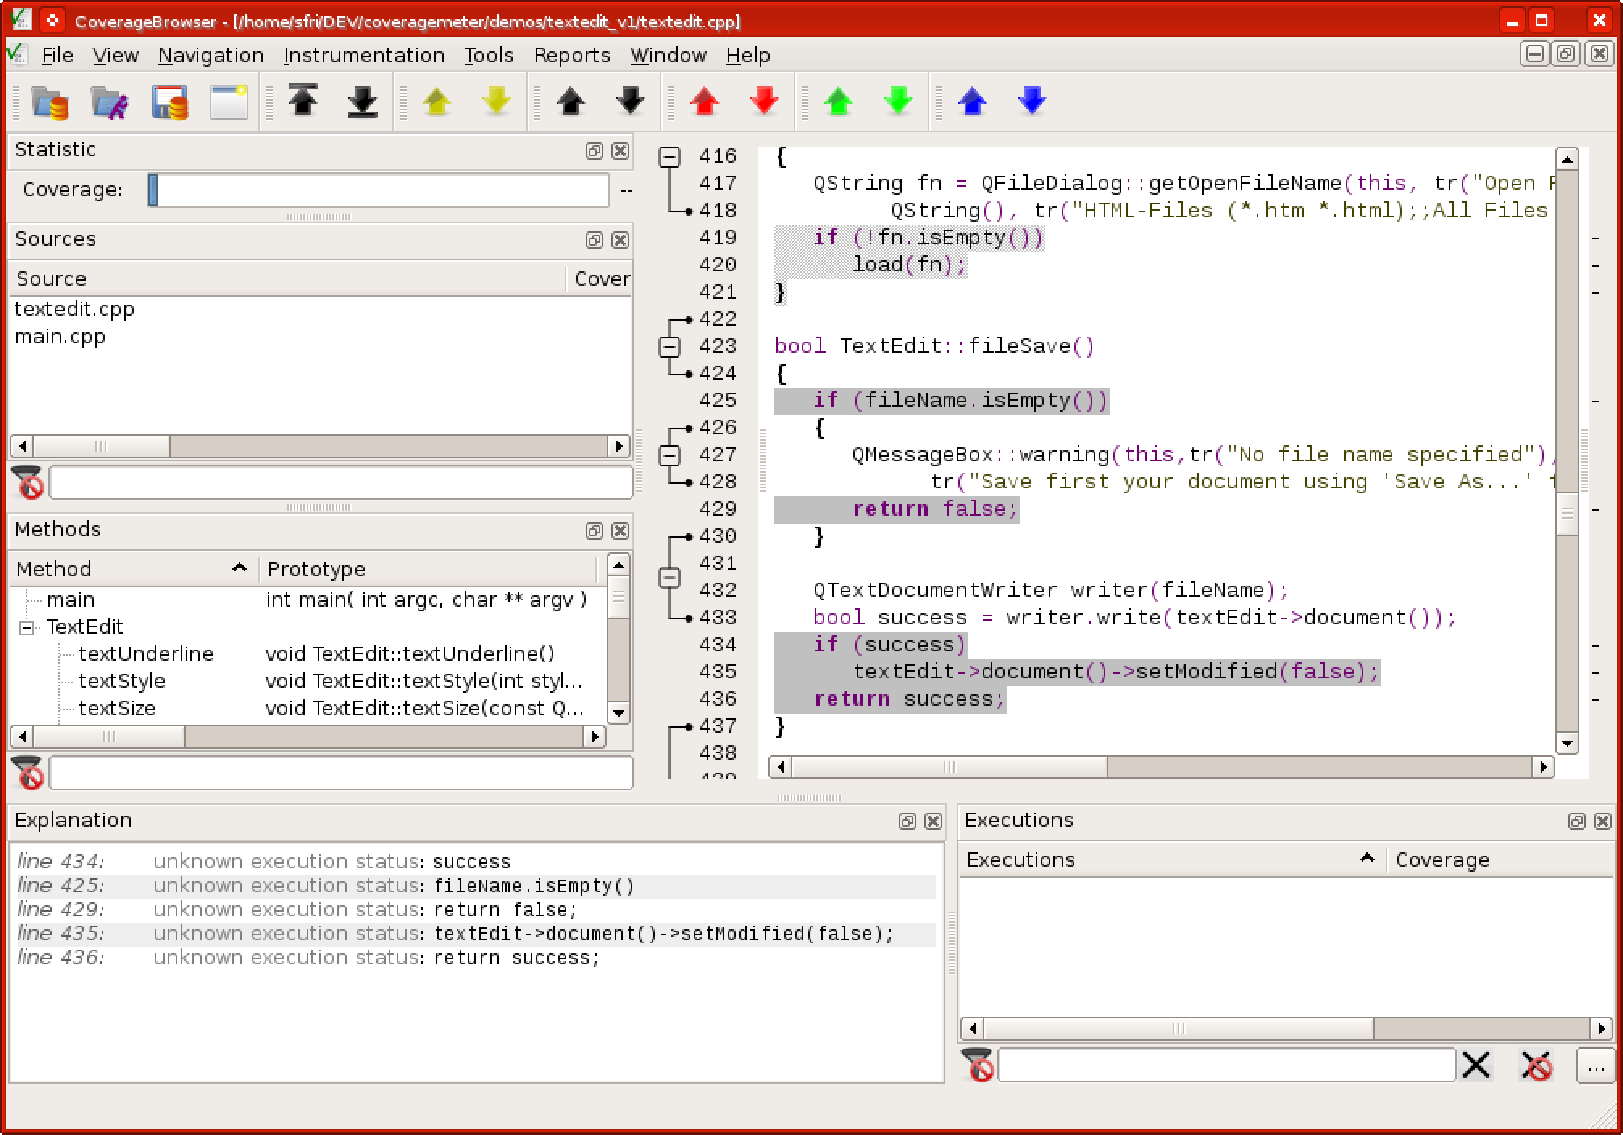
\includegraphics[scale=.5]{coveragebrowser_textedit}
  \end{center}
  \caption{\CoverageBrowser\ after loading \TextEdit\ instrumentation database}
  \label{fig:startup}
\end{figure}

By clicking on \GUIMenuTwo{File}{Load~Execution~Report\ldots}, 
an import dialog appears in which it is necessary to enter at least  the file path of
\verb$textedit.csexe$ (field: 'File~Name') and set  the name of the test (Field: 'Name') to
'\textsf{Start~and~Exit}'.  Also, it is judicious to activate the option
'Delete~after~loading' because the report is no longer necessary after our
import and set 'When~file~becomes~modified' to 'Open~this~dialog' to get this
dialog opened automatically after each test execution.

After the import, the coverage information is now visible:
\begin{itemize}
  \item The coverage statistics for each source, method and for the whole
    application will now have been computed.
  \item The source window is now colored and displays in a green (resp.
    red) background the executed (resp. unexecuted) code part.
  \item The execution list contains now one selected item called
    '\textsf{Start~and~Exit}', our only test execution report.
\end{itemize}

\subsubsection{Interactive testing}

{\CoverageBrowser} indicates that the function \verb$TextEdit::fileSave()$ is not executed.
We will try to validate it interactively, guided by the code coverage analysis.

In the actual output of the source window, all source code lines are marked
with a background in red, which means that they have not been executed. \seelstref{lst:src1}

    \begin{figureenv}
  \scriptsize
\begin{alltt}
bool TextEdit::fileSave()
\{
\colorbox{red}{  if (fileName.isEmpty())}
  \{
    QMessageBox::warning(this,tr("No file name specified"),
      tr("Save first your document using 'Save As...' from the menu"),
      QMessageBox::Ok );
\colorbox{red}{    return false;}
   \}

  QTextDocumentWriter writer(fileName);
  bool success = writer.write(textEdit->document());
\colorbox{red}{  if (success)}
\colorbox{red}{     textEdit->document()->setModified(false);}
\colorbox{red}{  return success;}
\}
\end{alltt}
\caption{{\CoverageBrowser} source view of the function TextEdit::save()}
\label{lst:src1}
\end{figureenv}

The first test we need to execute:
\begin{enumerate}
  \item start {\TextEdit},
  \item click on the '\textsf{Save}' button: {\TextEdit} displays the error message "Save
    first your document using 'Save As\ldots' from the menu"
  \item and quit.
\end{enumerate}

After importing the coverage report, {\CoverageBrowser} indicates that the '\verb$return false;$'
line just after the call of \verb$QMessageBox::warning()$ has been executed (line
    marked with a green background). But the line '\verb$if (fileName.isEmpty())$' is
marked as partially executed (orange background, \seelstref{lst:src2}.

\begin{figureenv}
  \scriptsize
\begin{alltt}
bool TextEdit::fileSave()
\{
\colorbox{orange}{  if (fileName.isEmpty())}
  \{
    QMessageBox::warning(this,tr("No file name specified"),
      tr("Save first your document using 'Save As...' from the menu"),
      QMessageBox::Ok );
\colorbox{green}{    return false;}
   \}

  QTextDocumentWriter writer(fileName);
  bool success = writer.write(textEdit->document());
\colorbox{red}{  if (success)}
\colorbox{red}{     textEdit->document()->setModified(false);}
\colorbox{red}{  return success;}
\}
\end{alltt}
\caption{{\CoverageBrowser} source view  after clicking on the 'Save' button of TextEdit.}
\label{lst:src2}
\end{figureenv}

The explanation window \seelstref{lst:src3} gives the information that the
evaluation of the expression '\verb$fileName.isEmpty()$' was true during one execution
but was never false. In order to fulfil this condition it is necessary to click
on  the '\textsf{Save As\ldots}' button,  to set the file name and then
click on the '\textsf{Save}' button.

\begin{figureenv}
  \scriptsize
  \textcolor{orange}{partially executed}: \texttt{fileName.isEmpty()} \par
\hspace{1cm}
\begin{tabularx}{9cm}{||X||X||} \hline\hline
  \begin{center}\textbf{TRUE}\end{center}          & \begin{center}{\textbf{FALSE}}\end{center}      \\ \hline\hline
  \centerline{\textcolor{green}{yes}} 
  \textit{Execution Count:} 1         \newline
  \textit{Executed by:}               \newline
  \hspace{.4cm}- Save Clicked         &

                                        \centerline{\textcolor{red}{no}} 
                                        \textit{Execution Count:} 0      
                                                                         \\ \hline\hline
\end{tabularx}
\caption{{\CoverageBrowser} explanation window after clicking on the 'Save' button of TextEdit.}
\label{lst:src3}
\end{figureenv}

After importing the new execution report only one source code line remains
partially untested \seelstref{lst:src4}. In this case, \CoverageBrowser\ indicates
that the boolean variable '\verb$success$' was never false, this means that writing
the document never fails. Of course it is possible to generate such write failures
and so achieve a 100\% code coverage of this function, but we will choose
another test strategy: implement a unit test and import the execution result
into {\TextEdit} instrumentation database.

\begin{figureenv}
  \scriptsize
\begin{alltt}
bool TextEdit::fileSave()
\{
\colorbox{green}{  if (fileName.isEmpty())}
  \{
    QMessageBox::warning(this,tr("No file name specified"),
      tr("Save first your document using 'Save As...' from the menu"),
      QMessageBox::Ok );
\colorbox{green}{    return false;}
   \}

  QTextDocumentWriter writer(fileName);
  bool success = writer.write(textEdit->document());
\colorbox{red}{  if (success)}
\colorbox{green}{     textEdit->document()->setModified(false);}
\colorbox{green}{  return success;}
\}
\end{alltt}
\caption{{\CoverageBrowser} source view  after clicking on the 'SaveAs\ldots' and 'Save' button of {\TextEdit}.}
\label{lst:src4}
\end{figureenv}


\subsubsection{Writing unit tests}

Writing a unit test which sets an illegal filename and execute \verb$fileSave()$ using
\QTestLib\ is pretty easy \seelstref{lst:src5}.

\begin{figureenv}
  \scriptsize
\begin{verbatim}
#include "tst_textedit.h"

void TestTextEdit::tst_saveFile() {
  TextEdit textEdit;
  textEdit.fileName="/";
  QVERIFY( ! textEdit.fileSave() );
}

QTEST_MAIN(TestTextEdit);
\end{verbatim}
\caption{{\TextEdit} unit test}
\label{lst:src5}
\end{figureenv}

To get the instrumentation result of this test into TextEdits own
instrumentation database, the following strategy can be applied:
\begin{enumerate}
  \item Create a {\qmake} project file with code coverage configured identically as for the {\TextEdit}
    project. 
  \item Add a post build rule which automatically executes the test and collects
    the coverage information.
  \item Add a unit test listener which saves into the unit tests own instrumentation database
    the code coverage data and the test status (passed or failed) for each unit test executed.
  \item Import the code coverage report into the {\TextEdit} instrumentation database.
\end{enumerate}

The unit test recompiles itself, and \texttt{textedit.cpp}. To be importable into the \TextEdit\
instrumentation database it is necessary that both  objects (this one from
{\TextEdit} and this one from the unit test) are  identically instrumented.
So we need first to use the same instrumentation option: \verb$--cs-count$,
\verb$--cs-full-instrumentation$ and \verb$--cs-qt4$.

This is unfortunately not enough because per default only source and header
files from the current directory are instrumented. We need to instrument the folder of
{\TextEdit} sources: this is achieved by using the \verb$--cs-include-path$ command line option.

This gives us the {\qmake} project file shown in \ref{lst:qmake3} which generates
the executable \texttt{tst\_textedit.exe} which then produces the execution report
\texttt{tst\_textedit.csexe}. This can be imported into \texttt{tst\_textedit.exe.csmes}
using \CoverageBrowser.

\begin{figureenv}
  \scriptsize
\begin{verbatim}
HEADERS         = ../textedit_v1/textedit.h \
                  tst_textedit.h

SOURCES         = ../textedit_v1/textedit.cpp \
                  tst_textedit.cpp

TestCocoon {
 TESTCOCOON_OPTIONS =  --cs-count --cs-full-instrumentation
 TESTCOCOON_OPTIONS += --cs-qt4
 TESTCOCOON_OPTIONS += --cs-output=tst_textedit
 TESTCOCOON_OPTIONS += --cs-include-path=../textedit_v1
 TESTCOCOON_OPTIONS += --cs-exclude-file-regex=qrc_.*

 QMAKE_CXXFLAGS += $$TESTCOCOON_OPTIONS
 QMAKE_CCFLAGS  += $$TESTCOCOON_OPTIONS
 QMAKE_LFLAGS   += $$TESTCOCOON_OPTIONS

 QMAKE_CC=cs$$QMAKE_CC
 QMAKE_LINK=cs$$QMAKE_LINK
 QMAKE_CXX=cs$$QMAKE_CXX
}

\end{verbatim}
\caption{Basic {\qmake} project file for unit test}
\label{lst:qmake3}
\end{figureenv}

We can automatically execute and import the execution report using a post build
rule. \TestCocoon\ provides on the side a command line tool call \cmcsexeimport\
which import an execution report into an instrumentation database.
The post build rule consists to delete first a previous executed report,
execute the test itself, and finally import it into the execution database of
\verb$tst_textedit$ \seelstref{lst:qmake4}.


\begin{figureenv}
  \scriptsize
\begin{verbatim}
TestCocoon {
 unix {
   QMAKE_POST_LINK  = rm tst_textedit_v1.csexe ;
   QMAKE_POST_LINK += ./tst_textedit_v1 ;
   QMAKE_POST_LINK += cmcsexeimport -m tst_textedit_v1.csmes \
                      -e tst_textedit_v1.csexe -t UnitTest
 }
 win32 {
   QMAKE_POST_LINK  = del /F tst_textedit_v1.csexe &
   QMAKE_POST_LINK += tst_textedit_v1.exe &
   QMAKE_POST_LINK += cmcsexeimport -m tst_textedit_v1.exe.csmes \
                      -e tst_textedit_v1.csexe -t UnitTest
 }
}
\end{verbatim}
\caption{Post build rules: importing execution report into unit test's instrumentation database}
\label{lst:qmake4}
\end{figureenv}

The actual implementation imports coverage data without any information about
the executed tests: an execution called '\textsf{UnitTest}' is created which does
not described which test was executed and if its execution was successful.
To provide this information it is necessary to use the \CoverageScanner\ API to
generate an execution report upon the execution of each test. A sample is
available on the \TestCocoon\
homepage\footnote{\url{http://testcocoon.org/testcoverageobject.cpp} and
\url{http://testcocoon.org/testcoverageobject.h}}. Using it is easy: 
\begin{itemize}
  \item Add the two source files in \qmake\ project file \seelstref{lst:qmake5}.
  \item Instead of inheriting the unit test from \texttt{QObject}, inherit it
    from \texttt{TestCoverageObject} \seelstref{lst:hdr1}.
\end{itemize}

\begin{figureenv}
  \scriptsize
\begin{verbatim}
HEADERS += testcoverageobject.h
SOURCES += testcoverageobject.cpp
\end{verbatim}
\caption{Including \CoverageScanner\ listener into {\qmake} project file}
\label{lst:qmake5}
\end{figureenv}

\begin{figureenv}
  \scriptsize
\begin{verbatim}
#include "testcoverageobject.h"
#include "../textedit_v1/textedit.h"
#include <QtTest/QtTest>

class TestTextEdit : public TestCoverageObject
{
    Q_OBJECT
  private slots:
    void tst_saveFile();
};
\end{verbatim}
\caption{\TextEdit\ unit test header}
\label{lst:hdr1}
\end{figureenv}

A small look in \texttt{testcoverageobject.cpp} \seelstref{lst:src6} lets
us understand how it works: it only provides a \verb$cleanup()$ function to
\QTestLib, which is executed after each unit test item.
The code between \verb$#ifdef __COVERAGESCANNER__$ and \verb$#endif$ is 
compiled when \CoverageScanner\ is invoked\footnote{\texttt{\_\_COVERAGESCANNER\_\_} define
is set automatically when using \CoverageScanner\ and so does not need to be
defined}. It builds a test name using the object name and the test function
name. In our case, an execution item \verb$unittest/TestTextEdit/tst_saveFile$
is generated. The slash permits to organize the tests in a tree view.
The current test status (``PASSED'' or ``FAILED'') is recorded, and
committed to the execution report by calling \verb$__coveragescanner_save()$.


\begin{figureenv}
  \scriptsize
\begin{verbatim}
.....
void TestCoverageObject::cleanup()
{
  cleanupTest();
#ifdef __COVERAGESCANNER__
  QString test_name="unittest/";
  test_name+=metaObject()->className();
  test_name+="/";
  test_name+=QTest::currentTestFunction();
  __coveragescanner_testname(test_name.toLatin1());
  if (QTest::currentTestFailed())
    __coveragescanner_teststate("FAILED"); 
  else 
    __coveragescanner_teststate("PASSED") ; 
  __coveragescanner_save();
  __coveragescanner_testname(""); 
#endif
}
\end{verbatim}
\caption{\texttt{TestCoverageObject} source code}
\label{lst:src6}
\end{figureenv}

At this stage we could start \CoverageBrowser, load the \TextEdit\ instrumentation
database and import the instrumentation database of the unit test
\GUIMenuTwo{File}{Import Unit Tests\ldots}, but we can also use \cmmerge\ to
automate this step. \cmmerge\ permits us  to import the execution report from one
instrumentation database into another. So it is possible to call it in
the post build rules to import the coverage information into \TextEdit\
database automatically \seelstref{lst:qmake6}.

\begin{figureenv}
  \scriptsize
\begin{verbatim}
TestCocoon {
 # Merge coverage database into TextEdit database
 unix {
   QMAKE_POST_LINK += ;
   QMAKE_POST_LINK += cmmerge -o ../textedit_v1/textedit.tmp \
                   -i ../textedit_v1/textedit.csmes ./tst_textedit_v1.csmes &&
   QMAKE_POST_LINK += rm ../textedit_v1/textedit.csmes &&
   QMAKE_POST_LINK += mv ../textedit_v1/textedit.tmp ../textedit_v1/textedit.csmes 
 }
 win32 {
   QMAKE_POST_LINK += &
   QMAKE_POST_LINK += cmmerge -o ../textedit_v1/textedit.tmp \
                   -i ../textedit_v1/textedit.csmes ./tst_textedit_v1.csmes &&
   QMAKE_POST_LINK += DEL /F ../textedit_v1/textedit.csmes &&
   QMAKE_POST_LINK += REN ../textedit_v1/textedit.tmp ../textedit_v1/textedit.csmes 
 }
}
\end{verbatim}
\caption{Post build rules: merging instrumentation results into \TextEdit\ instrumentation database}
\label{lst:qmake6}
\end{figureenv}

After building the unit test, the function \verb$fileSave()$ is displayed as
100\% covered by CoverageBrowser and the execution list contains our 3 manual
tests and one unit test. \seefigref{fig:execlist1}

\begin{figure}[H]
  \begin{center}
    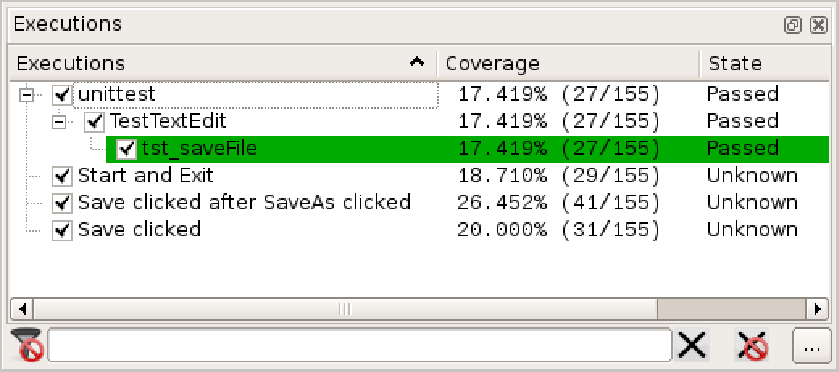
\includegraphics[scale=.5]{textedit_list_of_tests}
  \end{center}
  \caption{Execution list after execution of all tests}
  \label{fig:execlist1}
\end{figure}


\subsection{Working with code coverage data}

In most of the cases, the code coverage technology is only used by the
developer to find untested code portions and by the management to produce test
status diagrams. 

\TestCocoon\ provides some features which permit you to extend the application
area of the code coverage technique.


\subsubsection{Post mortem analysis}

Recording the coverage data of each test permits to compare it together and
answer the question: ``what does this test cover more than another?''. This is
particularly useful if one test fails and the developer wants to identify which
code part is involved.

For example, lets have a look at the \TextEdit\ sample. Clicking on '\textsf{Save}' generates
an error message telling us that no file name was defined. This is ergonomically
interesting since that
\TextEdit\ could also open directly the '\textsf{SaveAs\ldots}' dialog. 

To identify which code part is impacted, we simply compare the '\textsf{Save Clicked}'
execution to all other which involve the '\textsf{Save}' button. First it is necessary
to switch into the ``Execution Benefit Analysis'' mode
(Menu: \GUIMenuTwo{Tools}{Execution Benefit Analysis}). In the execution list select
the tests ``\textsf{tst\_saveFile}'' and ``\textsf{SaveAs clicked before Save clicked}''. Double
click on ``\textsf{Save clicked}'' execution: the execution comparison symbol appears in
front of its name \seefigref{fig:execlist2}.

\begin{figure}[H]
  \begin{center}
    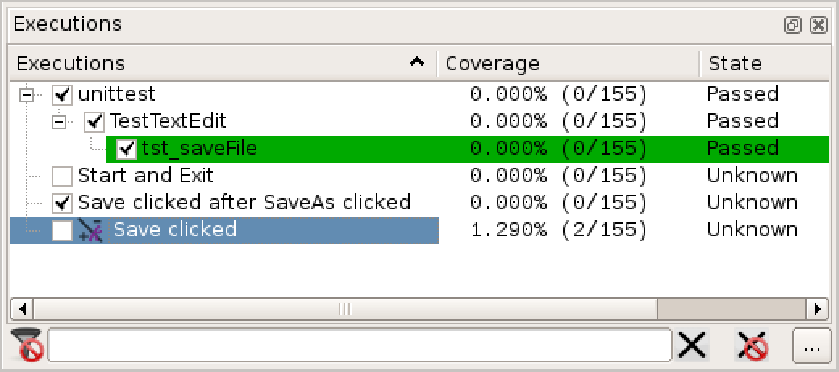
\includegraphics[scale=.5]{textedit_list_of_tests_benefit}
  \end{center}
  \caption{Execution list when comparing executions together}
  \label{fig:execlist2}
\end{figure}

In this mode the coverage analysis is made only on source code lines which are
not executed by ``\textsf{tst\_saveFile}'' and ``\textsf{SaveAs clicked before Save clicked}''.
That's why the overall coverage decreases to 1.3\% which means in this case
that ``\textsf{Save clicked}'' executes 1.3\% more code than the selected tests. 

A deeper look on the source code shows that  only two lines of the
\verb$TextEdit::fileSave()$ function \seelstref{lst:src10} are not grayed:
the lines which pop-up the error message. This are the lines that needs to be
modified to change the behaviour behind the ``\textsf{Save}'' button.

\begin{figureenv}
  \scriptsize
\begin{alltt}
bool TextEdit::fileSave()
\{
\colorbox{orange}{  if (fileName.isEmpty())}
  \{
    QMessageBox::warning(this,tr("No file name specified"),
      tr("Save first your document using 'Save As...' from the menu"),
      QMessageBox::Ok );
\colorbox{green}{    return false;}
   \}

  QTextDocumentWriter writer(fileName);
  bool success = writer.write(textEdit->document());
\colorbox{Graylight}{  if (success)}
\colorbox{Graylight}{     textEdit->document()->setModified(false);}
\colorbox{Graylight}{  return success;}
\}
\end{alltt}
\caption{{\CoverageBrowser} source view of the benefit of the execution ``Save clicked''.}
\label{lst:src10}
\end{figureenv}

Correcting the \verb$fileSave()$ function is trivial and consists only to
replace the call of \verb$QMessageBox::warning()$ through \verb$fileSaveAs()$.
\seelstref{lst:src11}

\begin{figureenv}
  \scriptsize
\begin{verbatim}
bool TextEdit::fileSave()
{
   if (fileName.isEmpty())
     return fileSaveAs();

   QTextDocumentWriter writer(fileName);
   bool success = writer.write(textEdit->document());
   if (success)
      textEdit->document()->setModified(false);
   return success;
}
\end{verbatim}
\caption{\TextEdit\ with a modified \texttt{fileSave()} function.}
\label{lst:src11}
\end{figureenv}

\subsubsection{\label{sec:patchimpact}Evaluation of the impact of a hot fix}

Before committing a change or starting to test a hot fix, it is possible to
estimate the impact of the code modification. \CoverageBrowser\ is able
to perform an analysis on the difference between two source sets and so lists
which tests are or are not impacted.

Start \CoverageBrowser\ and load the instrumentation database of the  original
\TextEdit\ sample. Then click on \GUIMenuTwo{Tools}{Compare with\ldots} and
select the modified version of \TextEdit\ instrumentation database.
\CoverageBrowser\ displays  now the source code like a text comparison
application.

Clicking on \GUIMenuTwo{Tools}{Analysis on Modified Methods} permits to exclude
all unmodified functions from the coverage analysis. In our case, it is as if
only the function \verb$TextEdit::fileSave()$ was instrumented. \seefigref{fig:patchimpact}
This also impacts the statistic calculations: the coverage statistic of an
execution is also limited only to this function. Some executions have now a
coverage statistic which is not zero, these tests are impacted by the code
modification we made. 

In our case:
\begin{itemize}
  \item ``Save clicked'',
  \item ``SaveAs clicked before Save clicked'' and 
  \item ``tst\_saveFile'' (our unit test).
\end{itemize}

``Start and Exit'' has a coverage equal to 0\% and so does not execute our
patched code.

In other words, only two manual tests and one unit test need to be re-executed
to ensure that no regressions are generated.

\begin{figure}[H]
  \begin{center}
    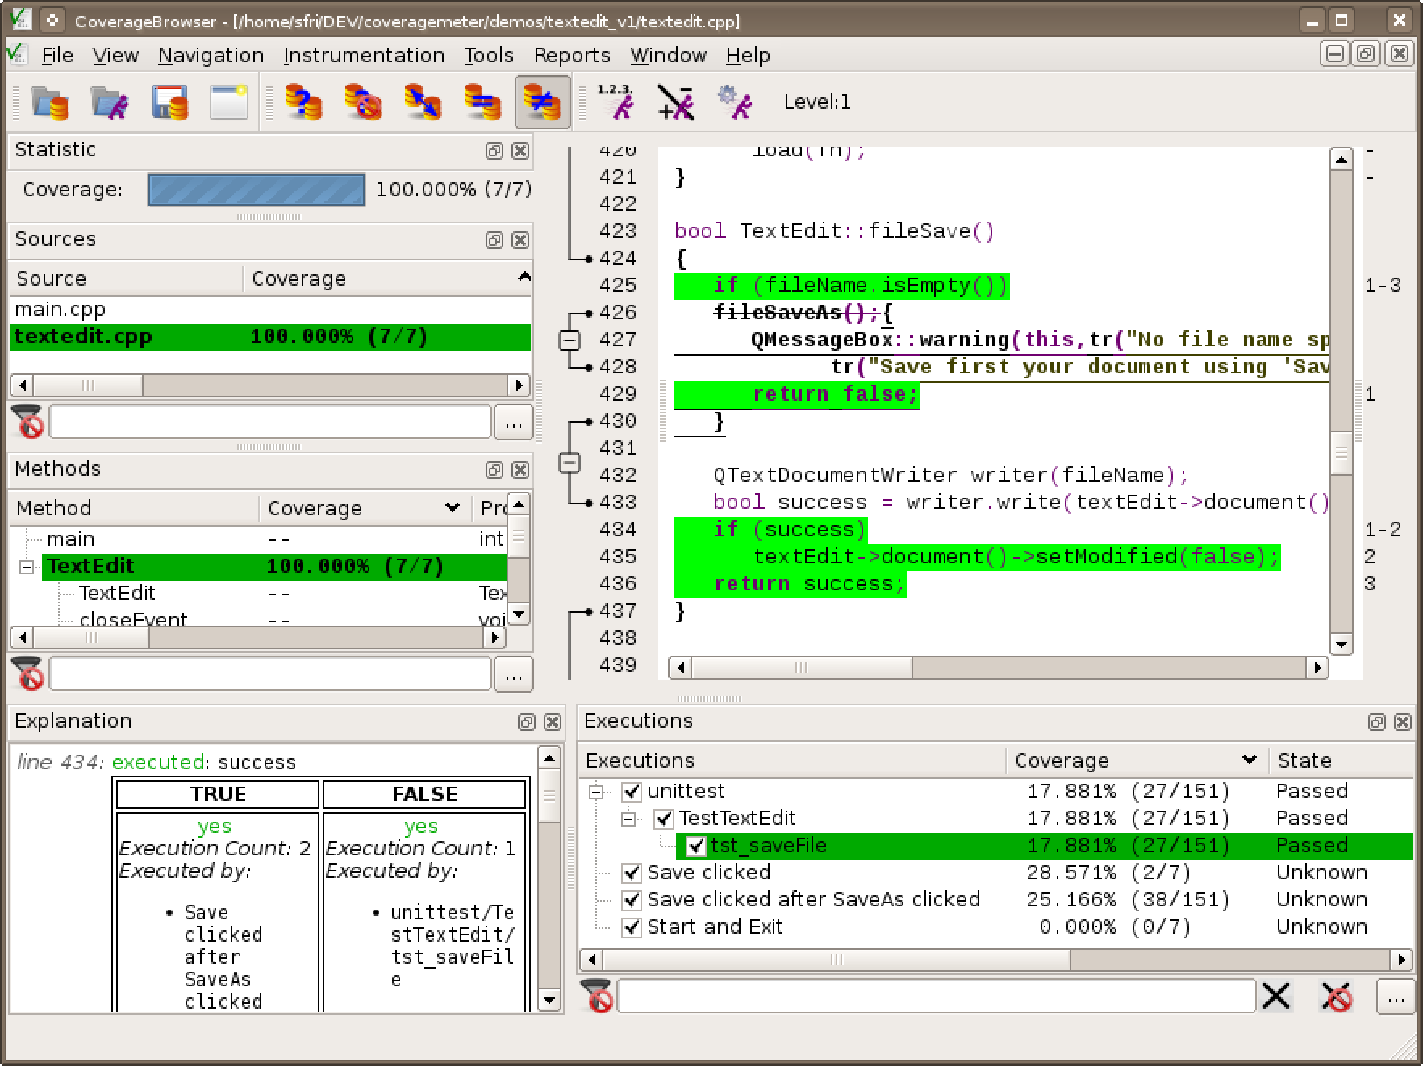
\includegraphics[scale=.5]{textedit_patch_impact}
  \end{center}
  \caption{List of tests impacted by a modification}
  \label{fig:patchimpact}
\end{figure}

\subsubsection{Black-box testing/distributed testing}

To test the new version of \TextEdit\ we decide to perform what is called  black-box testing.
This kind of testing consists of testing without having access to or knowledge of the code. But, contrary to what you would believe,
the code coverage analysis is still possible. 

\TestCocoon\ gives the possibility to generate a
black-box database which does not contain the source code. 
Simply click on \GUIMenuTwo{File}{Generate Black-Box Configuration\ldots} to
generate a new instrumentation database. This database, with \TextEdit\
executable, can be transmitted to the test team which can then use it with a
simplified version of \CoverageBrowser\ \seefigref{fig:blackbox}: only
importing and the managing execution report are possible.

\begin{figure}[h]
  \begin{center}
    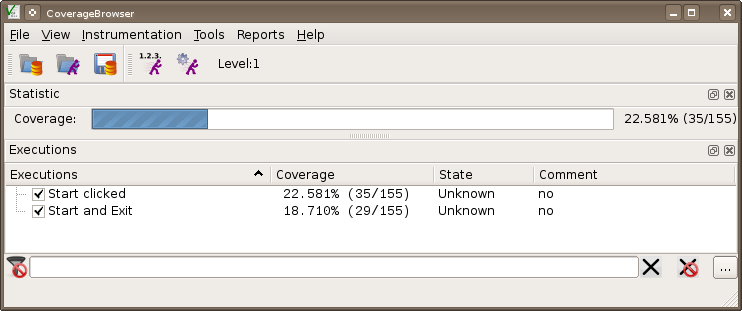
\includegraphics[scale=.5]{textedit_blackbox}
  \end{center}
  \caption{Black-box testing using \CoverageBrowser}
  \label{fig:blackbox}
\end{figure}


Once all tests are  finished, this black-box database can be merged into the original
\TextEdit\ database using \CoverageBrowser\ merge facilities (Menu:
\GUIMenuTwo{File}{Merge width\ldots}).

\subsubsection{Verifying if a bug fix is correctly tested}

Generally, when a small bug fix is made, the most important part of the source
code remains unchanged, and so retesting the whole application is generally not
necessary. \TestCocoon\ is able to work on only the modified source code
between two software versions\footnote{see \nameref{sec:patchimpact}, page
\pageref{sec:patchimpact}} and so focus the analysis on the patch. Simply
load the instrumentation database of the newest \TextEdit\ version, compare it
to the first version and activate the analysis on modified functions.

\begin{figure}[h]
  \begin{center}
    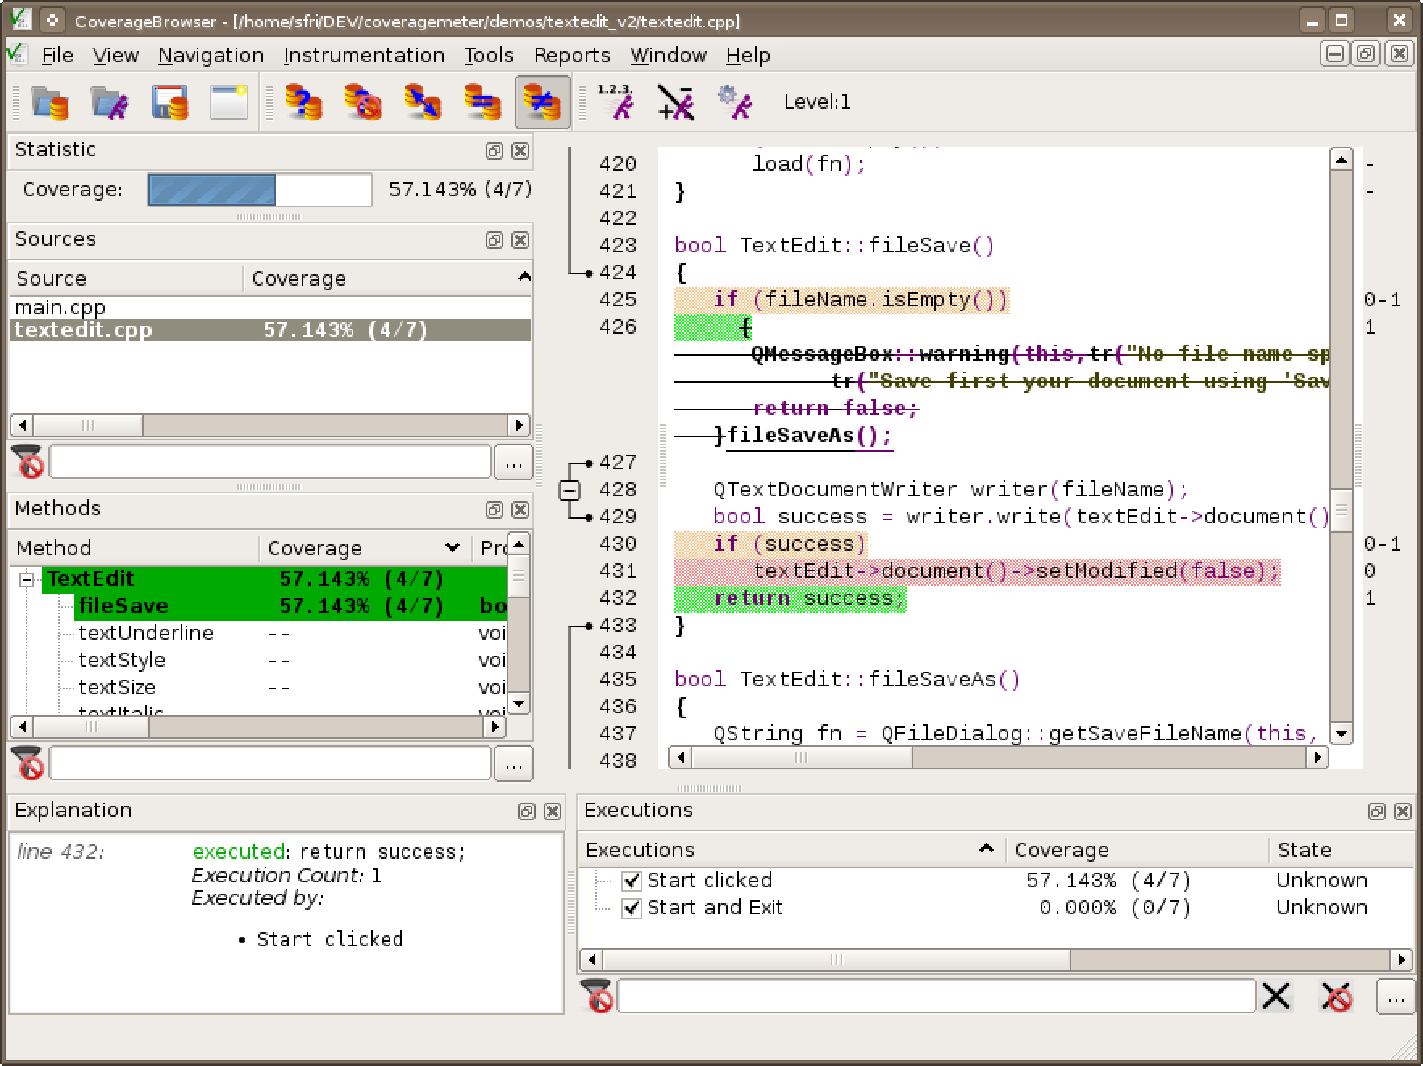
\includegraphics[scale=.5]{textedit_patch_coverage}
  \end{center}
  \caption{Coverage of the patched function}
  \label{fig:patchcoverage}
\end{figure}

The result is visible in \ref{fig:patchcoverage}: the two tests ``Start
clicked'' and ``Start and Exit'' are covering 57\% of
\verb$TextEdit::fileSave()$ function, the only modified method from our fix.

\section{Conclusion}

  \TestCocoon\ provides code coverage analysis which can be applied to
the majority of testing techniques: unit, manual and
black-box testing. Its analysis ignores the code generated by Qt tools 
(\moc, \qrc\ and \uic) and so instruments only the code generated by and of interest to
developers. The test results can be collected into one database
and can be used to evaluate the test progress of a complete application.
Also it helps to estimate the impact of a code
modification and measure the testing level of patch without retesting
the whole application again.

